\chapter{System Architecture}
\label{ch:architecture}

\section{Architectural Style}

\noindent The system uses three cooperating kinds of components as prescribed
by the design held throughout the project:

\begin{itemize}
  \item a \textbf{modular monolith API} (NestJS/TypeScript) that contains all
  business modules --- identity, tenancy, academic structure, content,
  materials, study, questions, examination, practice, jobs, export, and the
  OCR coordinator;
  \item \textbf{asynchronous workers} (Python and TypeScript) that consume
  RabbitMQ queues for material processing and AI generation;
  \item a \textbf{separately deployable OCR service} (FastAPI/Python) that
  performs vision-based extraction and can be scaled independently.
\end{itemize}

\noindent The API is deliberately \emph{not} split into microservices: the
business modules share one database connection pool and one deployment unit,
which keeps transactions, migrations, and authorization evaluation simple and
consistent, while the genuinely independent compute (OCR, AI) is delegated to
separate components.

\section{Deployment Topology}

\noindent Figure~\ref{fig:architecture} shows the deployment topology. The
only public ingress is a Cloudflare Tunnel through which all traffic flows to
an internal nginx reverse proxy. nginx splits the traffic by path: everything
under \texttt{/api/} is proxied to the API's internal port 3000 (with the
\texttt{/api/v1} prefix preserved), and the remaining paths go to the
Next.js web application on its internal port 3001. Postgres, Redis,
RabbitMQ, the OCR service, the workers, and the AI gateway are all internal
services that sit on the private Docker network and expose no host port.

\begin{figure}[h]
\centering
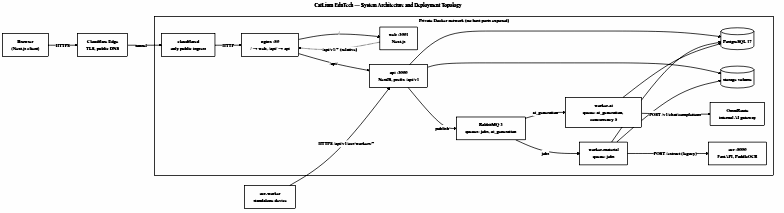
\includegraphics[width=\textwidth]{figures/system-architecture-bw.png}
\caption{System architecture and deployment topology.}
\label{fig:architecture}
\end{figure}

The web application sends its requests to the same origin path
\texttt{/api/v1/\ldots}, which nginx forwards to the API, so browsers never
address internal hosts directly. This single-boundary design means the browser
perceives one same-origin API, and no internal service needs to be publicly
reachable for any user-visible behaviour.

\section{Request Flow and Global Guards}

\noindent Every API request passes a global guard stack registered at the
application root before any controller logic runs:

\begin{enumerate}
  \item \texttt{ThrottlerGuard} --- global rate limit (default 100 requests
  per 60 seconds), tightened to 5 per 60 seconds on authentication routes.
  \item \texttt{CsrfGuard} --- double-submit CSRF check on every cookie-
  authenticated state-changing request.
  \item A global exception filter that normalizes errors into a consistent
  envelope.
\end{enumerate}

\noindent Per-controller, the authorization chain runs
\texttt{AccessTokenGuard $\rightarrow$ TenantGuard $\rightarrow$
RolesGuard $\rightarrow$ PermissionGuard $\rightarrow$ AcademicScope/evaluation
service}, detailed in Chapter~\ref{ch:security} and summarized in
Figure~\ref{fig:permission-model}.

\section{Asynchronous Processing}

\noindent Long-running work is never executed on the request thread. When the
API must perform heavy work it:

\begin{enumerate}
  \item writes a \texttt{jobs} row with status \texttt{queued},
  \item publishes a message to RabbitMQ (or, for coordinator-owned work,
  lets the coordinator sweep adopt it),
  \item returns \texttt{202 Accepted} with the job identifier, and
  \item lets the client poll the job status.
\end{enumerate}

\noindent Two RabbitMQ queues exist: \texttt{jobs} (material processing) and
\texttt{ai\_generation} (all AI operations), with the AI consumer running with
bounded concurrency. AI-related and extraction job types are reserved to
guarded paths; the public job endpoint accepts only material processing and
enhancement types, so a caller cannot forge a request that produces AI output
under another identity. The OCR pipeline is \emph{coordinator-owned}: the
in-API coordinator materialises page-range chunks, hands them to registered
OCR workers under a lease, and aggregates results (Chapter~\ref{ch:features}).
Figure~\ref{fig:ocr-processing} and Figure~\ref{fig:ocr-state} illustrate the
OCR flow and all job/chunk state transitions.

\section{AI Gateway}

\noindent All model calls pass through the internal \texttt{OmniRoute}
gateway, an OpenAI-compatible endpoint. Workers authenticate to the gateway
with their own endpoint key, and no application or worker code calls a cloud
AI provider directly. This keeps the provider switchable and the network
boundary simple.

\section{Health Endpoints}

\noindent The API exposes a health endpoint at
\texttt{GET /api/v1/health} (the global API prefix \texttt{/api/v1} applies to
all controllers). The OCR service exposes its own \texttt{GET /health} route
without an API prefix. These are used by the deployment to report service
liveness.